\chapter{Planificación}

Este capítulo establece el marco metodológico del proyecto. En primer lugar, se presentan la motivación e hipótesis y se delimita el problema a resolver. A continuación, se describe el proceso de diseño de software seguido (análisis, diseño, implementación y despliegue/validación), del que se derivan las tareas T1–T9 que estructuran el trabajo. Por último, se recoge la planificación temporal mediante un diagrama de Gantt y se incluye una estimación de costes.

%\section{Motivación e hipótesis}

%La motivación de este trabajo es reducir la barrera técnica para explorar MIMIC-IV mediante una plataforma web con visualizaciones y capacidades de IA. La hipótesis de partida es que un diseño cliente–servidor con API especializada, agregaciones optimizadas y asistencia de LLMs (resúmenes y consultas en lenguaje natural) permite a perfiles clínicos no técnicos extraer conocimiento útil del dataset de forma eficiente y segura.

\section{Problema a resolver}

Investigadores y personal sanitario carecen de interfaces abiertas y mantenidas para explorar MIMIC-IV sin escribir consultas. El problema concreto es construir una solución accesible, con rendimiento adecuado sobre datos voluminosos, que integre visualizaciones clínicas relevantes y soporte IA de forma controlada.

\section{Proceso de diseño de software}

El proyecto se estructura como un proceso clásico de ingeniería de software con cuatro fases: (1) análisis, (2) diseño, (3) implementación y (4) despliegue/validación. Cada fase produce artefactos alineados con la solución:
\begin{itemize}
  \item \textbf{Análisis}: requisitos (RF/RNF), actores y casos de uso; estudio del dataset y limitaciones.
  \item \textbf{Diseño}: arquitectura cliente–servidor, modelo de datos y API, y diseño de vistas.
  \item \textbf{Implementación}: carga y organización de datos, servicio de API, visualizaciones y módulo de IA.
  \item \textbf{Despliegue y validación}: publicación, demo y vídeo, pruebas exploratorias.
\end{itemize}

\section{Derivación de tareas desde los objetivos}

De los objetivos del Capítulo~1 (OE1–OE7) se derivan las siguientes tareas:

\begin{enumerate}
  \item \textbf{T1 (OE1)} Análisis inicial: revisión del estado del arte, estudio del dataset y criterios de selección tecnológica.
  \item \textbf{T2 (OE2)} Ingesta MIMIC-IV (demo): preparación de entorno, importación y validación.
  \item \textbf{T3 (OE2)} Ingesta MIMIC-IV (completa): indexación, colecciones preagregadas y optimización de consultas.
  \item \textbf{T4 (OE3)} API núcleo: endpoints de pacientes y dashboard con tests básicos de respuesta.
  \item \textbf{T5 (OE3)} API de visualizaciones: endpoints específicos para las visualizaciones planificadas.
  \item \textbf{T6 (OE4)} Frontend base: páginas (home, dashboard, paciente, chat) y componentes de interfaz.
  \item \textbf{T7 (OE4)} Visualizaciones: implementación y validación de las gráficas interactivas.
  \item \textbf{T8 (OE5)} IA: resúmenes de paciente y chat en lenguaje natural sobre los datos.
  \item \textbf{T9 (OE6–OE7)} Despliegue y demo: publicación, vídeo de demostración y enlaces finales.
\end{enumerate}

Se presenta un diagrama de Gantt que recoge la planificación temporal del proyecto, abarcando los meses de marzo a agosto. El diagrama refleja las tareas derivadas de los objetivos expuestos, y permite visualizar la distribución y el solapamiento de actividades a lo largo de todo el desarrollo.

\begin{figure}[H]
    \centering
    \fbox{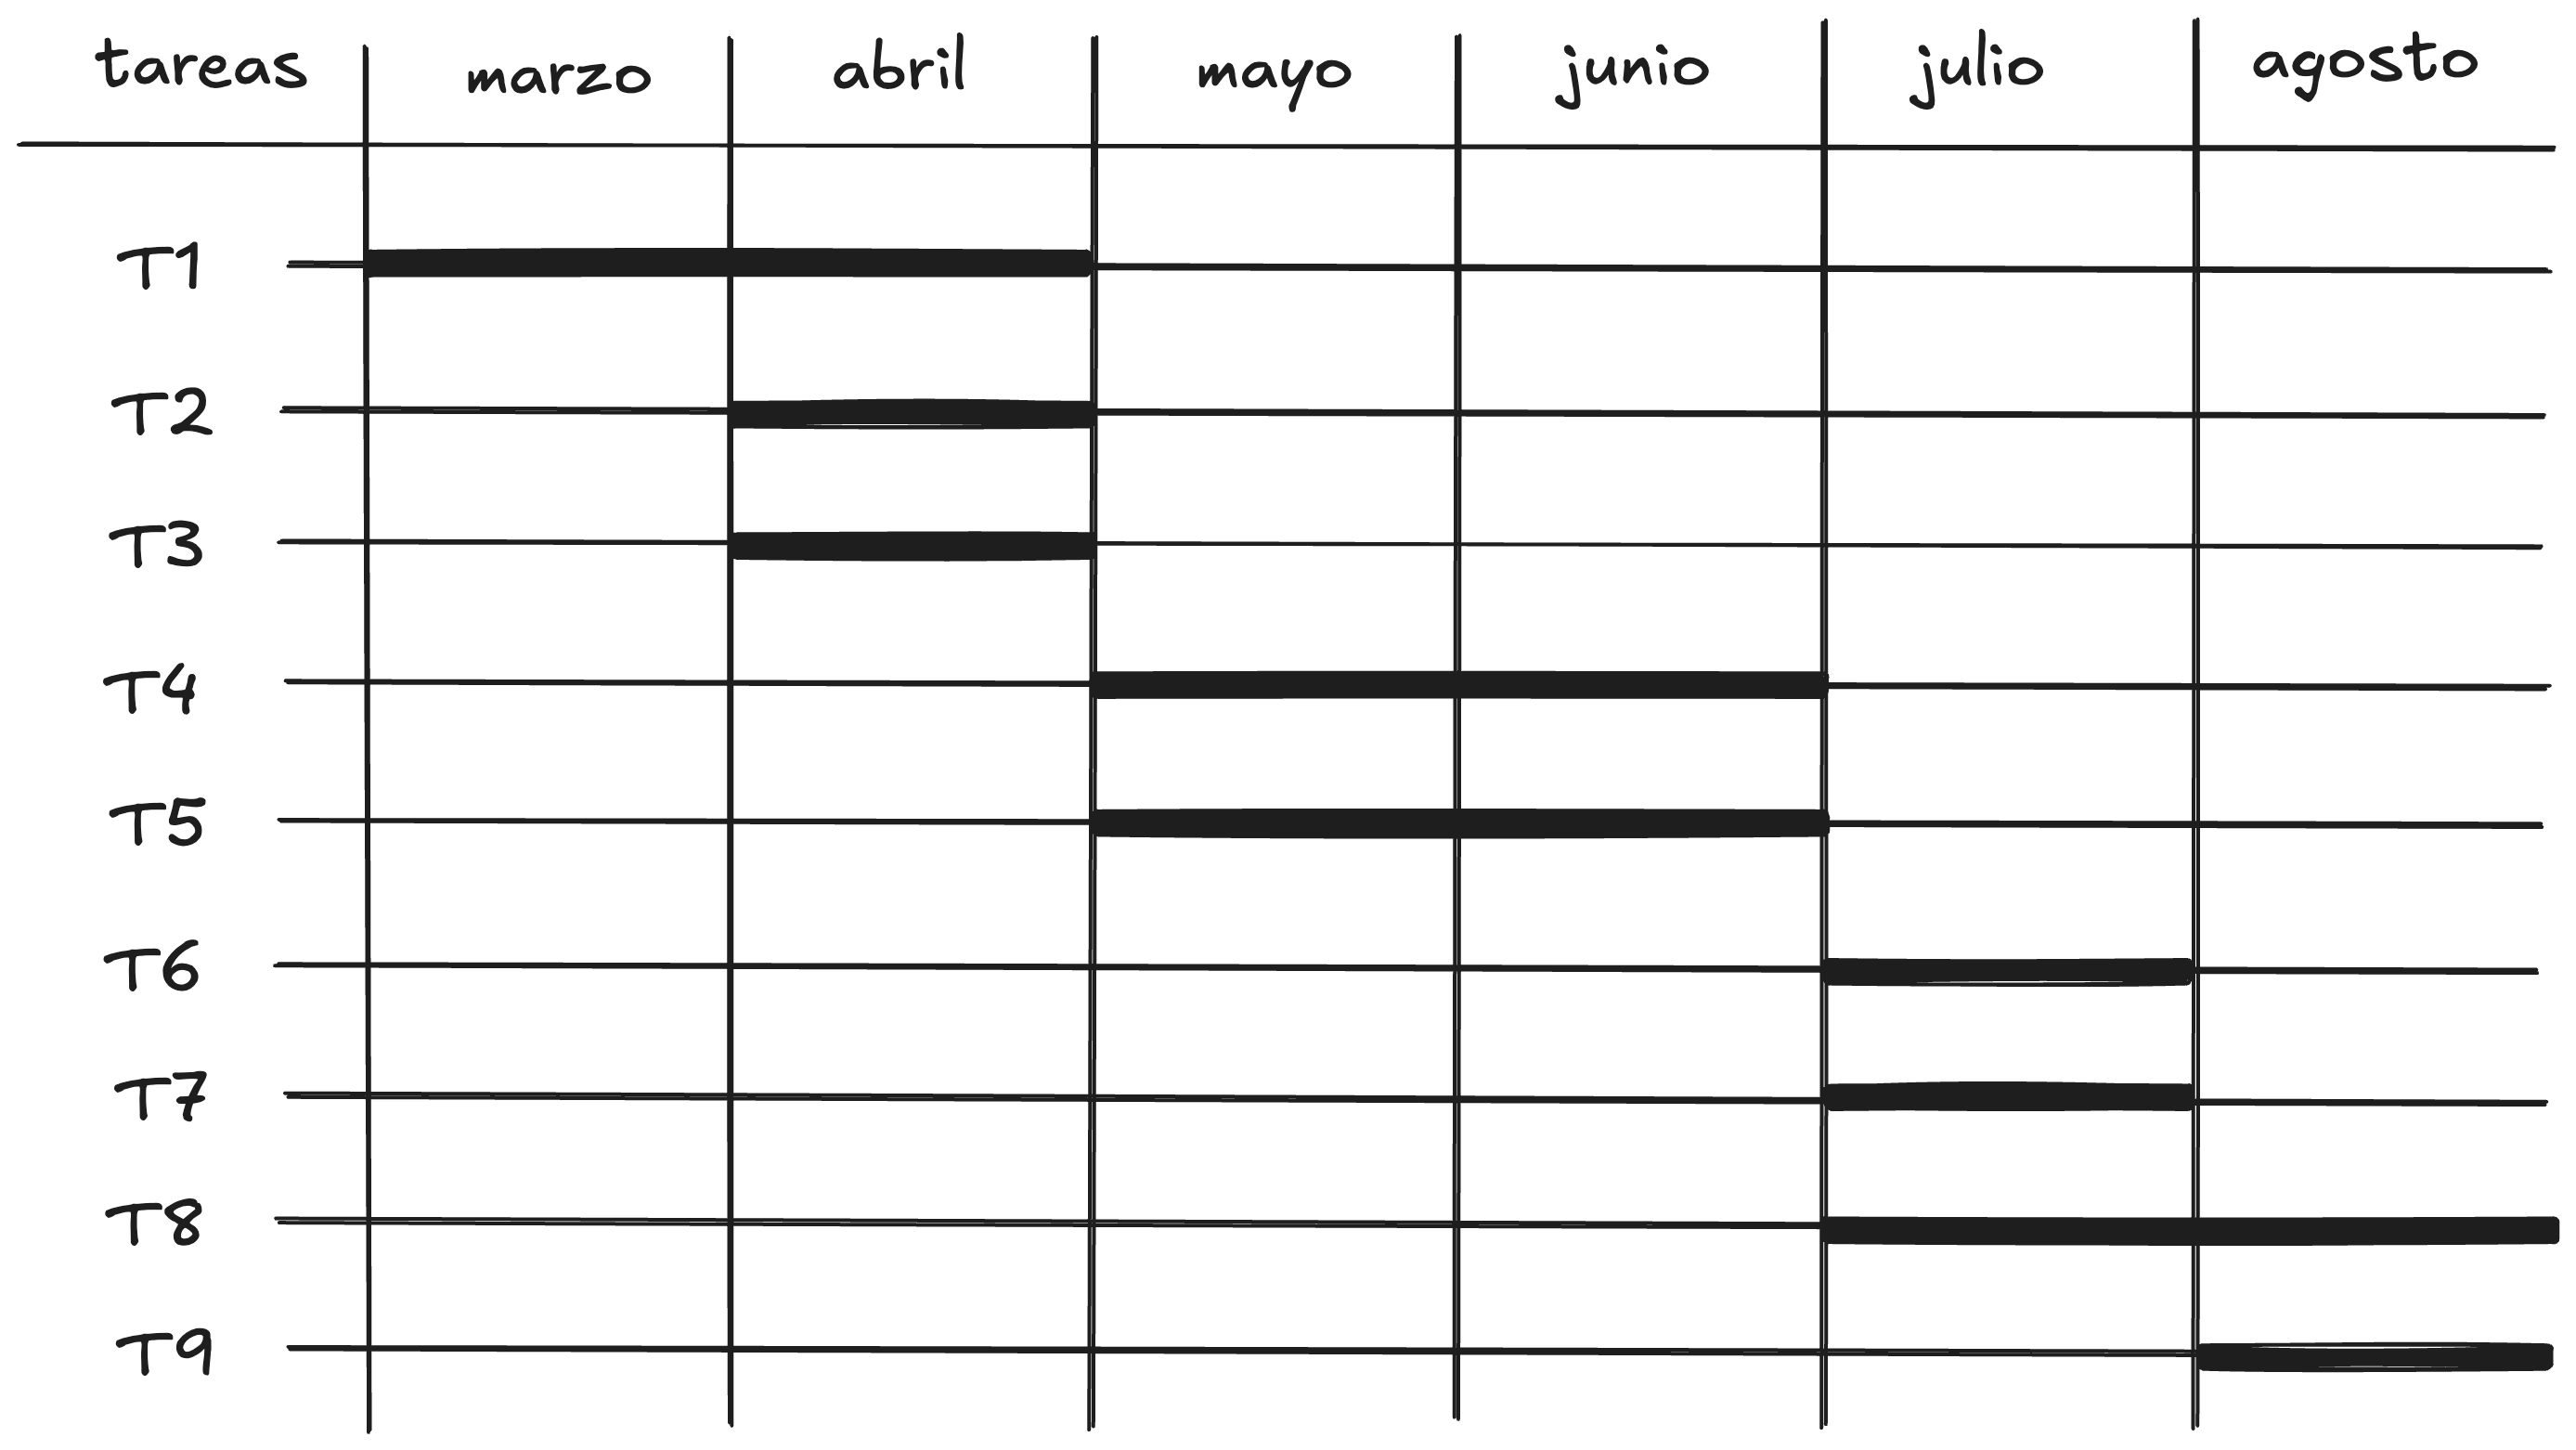
\includegraphics[width=\textwidth]{imagenes/gantt3.png}}
    %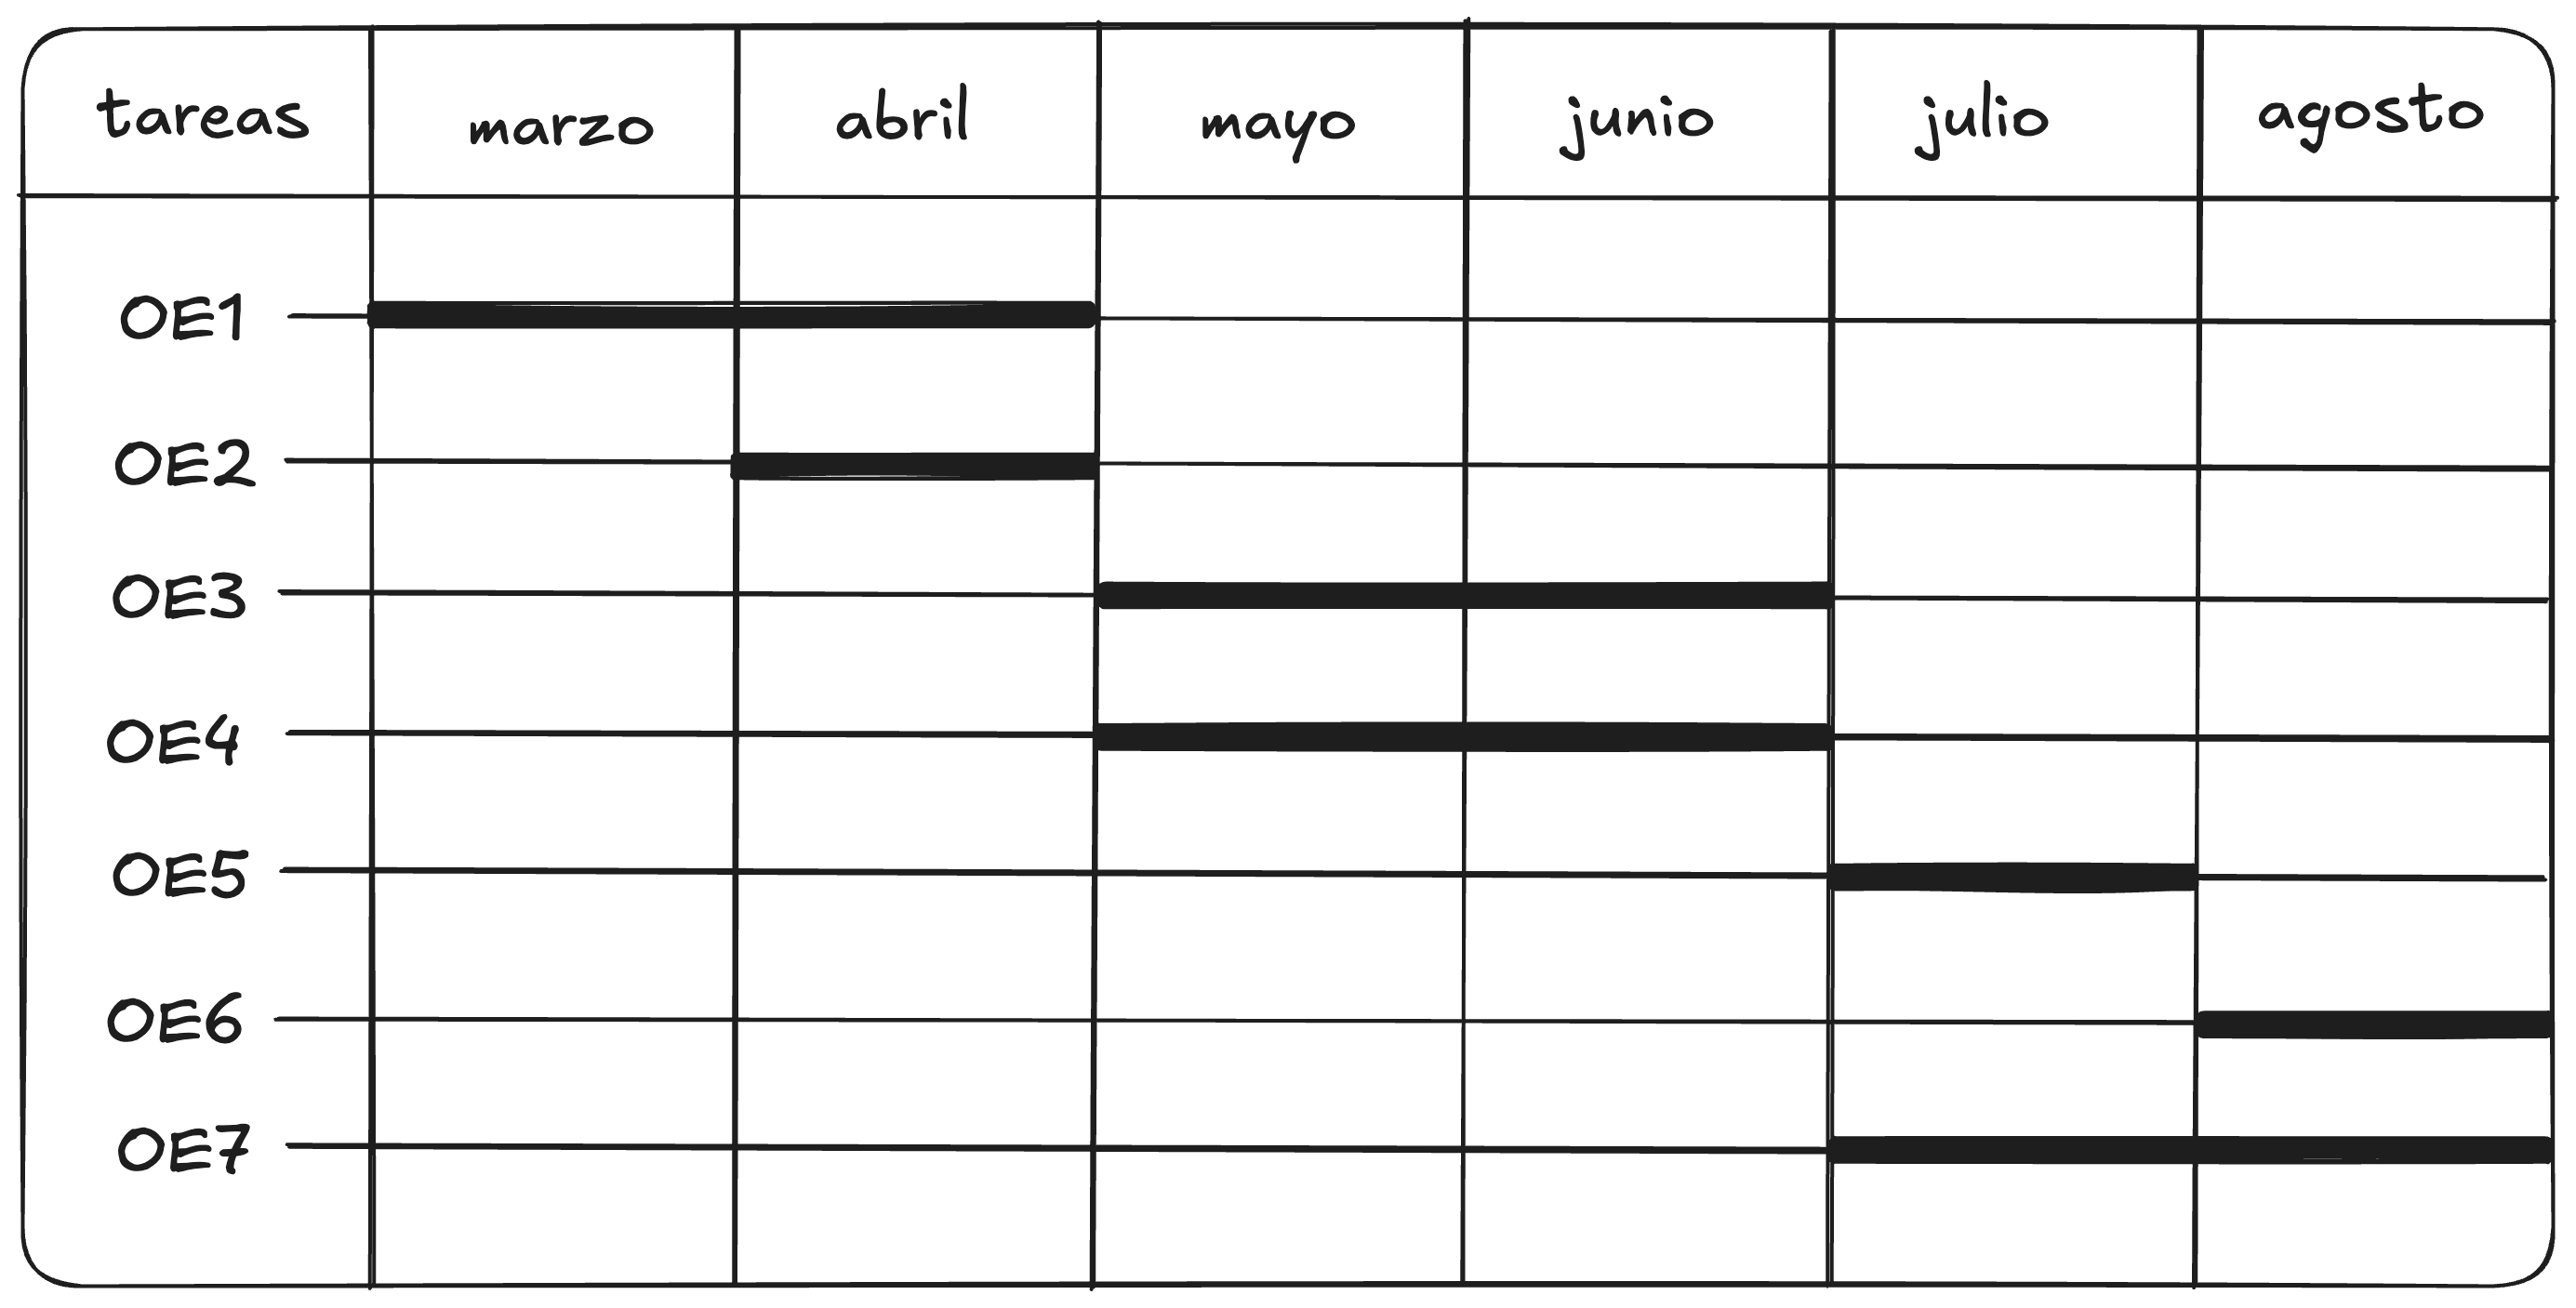
\includegraphics[width=\textwidth]{imagenes/gantt1.png}
    \caption{Diagrama de Gantt con la planificación del proyecto.}
\end{figure}

\section{Costes}

Si bien este proyecto tiene un enfoque académico, la elaboración de un presupuesto permite obtener una perspectiva más objetiva sobre el trabajo realizado. Este ejercicio aporta tanto un marco técnico como económico, acercando la iniciativa a escenarios reales y facilitando estimaciones útiles para futuras implementaciones o propuestas. Asimismo, contribuye a fundamentar las decisiones técnicas en función de su viabilidad financiera.

Para la estimación de costes, se han tenido en cuenta los recursos humanos, el equipamiento tecnológico y las herramientas de software empleadas. El cálculo se apoya en las tarifas promedio del sector de la programación en España y en los recursos técnicos requeridos. Los datos salariales se han extraído de la plataforma Glassdoor \cite{glassdoor}. Se ha considerado una duración total del proyecto de cinco meses.

\subsubsection{Costes humanos}

En un proyecto de software realista, además de un desarrollador junior a jornada completa, es habitual contemplar la participación parcial de un desarrollador senior (diseño, revisión y mentoría). Las tarifas se justifican con salario anual medio en España (fuente: Glassdoor \cite{glassdoor}), convertido a coste por hora asumiendo 2.016 horas/año (8 h/día \(\times\) 21 días/mes \(\times\) 12 meses).

\paragraph{Perfiles y salarios anuales medios (justificación).}
\begin{itemize}
  \item Desarrollador junior: 20.000\,€/año $\Rightarrow$ 20.000 / 2.016 $\approx$ 9,92\,€/hora.
  \item Desarrollador senior: 40.000\,€/año $\Rightarrow$ 40.000 / 2.016 $\approx$ 19,84\,€/hora.
\end{itemize}

\paragraph{Cálculo de costes.}
\noindent\textbf{Desarrollador junior (tiempo completo)}\\
\[
\text{Coste mensual} = 9{,}92\,€/h \times 168\,\text{h/mes} = 1.666{,}56\,€
\]
\[
\text{Coste total (5 meses)} = 1.666{,}56\,€ \times 5 = 8.332{,}80\,€
\]

\noindent\textbf{Desarrollador senior (mentoría y revisión, 4 h/semana)}\\
\[
\text{Horas totales} = 4\,\text{h/sem} \times 4\,\text{sem/mes} \times 5\,\text{meses} = 80\,\text{h}
\]
\[
\text{Coste senior} = 19{,}84\,€/h \times 80\,\text{h} = 1.587{,}20\,€
\]

\paragraph{Resumen de coste de personal.}
\[
\text{Personal} = 8.332{,}80\,€ + 1.587{,}20\,€ = \mathbf{9.920{,}00\,€}
\]

\subsubsection{Costes de material}

Para el desarrollo del proyecto se han utilizado los siguientes equipos. Dado que el hardware tiene una vida útil superior a la duración del proyecto, se ha calculado el coste imputable en función del tiempo de uso exclusivo para este trabajo (5 meses, aproximadamente 0,42 años):

\begin{center}
\begin{tabular}{|l|c|c|c|}
\hline
\textbf{Material} & \textbf{Precio compra (€)} & \textbf{Vida útil (años)} & \textbf{Coste imputable (€)} \\
\hline
Ordenador portátil & 2.000 & 4 & 210,00 \\
Servidor doméstico & 500 & 5 & 42,00 \\
\hline
\multicolumn{3}{|r|}{\textbf{Total}} & \textbf{252,00} \\
\hline
\end{tabular}
\end{center}

\noindent El cálculo del coste imputable sigue la fórmula:
\begin{equation*}
\text{Coste imputable} = \frac{\text{Precio de compra}}{\text{Vida útil (años)}} \times \text{Tiempo de uso (años)}
\end{equation*}

\subsubsection{Costes de herramientas}

Todo el software empleado en el desarrollo del proyecto corresponde a herramientas de licencia gratuita o planes gratuitos, por lo que no suponen coste adicional. No obstante, se ha utilizado la API de OpenAI con un coste total de 20€, además de un dominio personalizado con coste de 10€.

\begin{center}
\begin{tabular}{|l|c|}
\hline
\textbf{Herramienta} & \textbf{Coste (€)} \\
\hline
Software (licencias gratuitas) & 0 \\
Dominio & 10 \\
API OpenAI & 20 \\
\hline
\textbf{Total} & \textbf{30} \\
\hline
\end{tabular}
\end{center}

\subsubsection{Resumen de costes}

A continuación se muestra un resumen de todos los costes estimados para el proyecto:

\begin{center}
\begin{tabular}{|l|c|}
\hline
\textbf{Concepto} & \textbf{Coste (€)} \\
\hline
Coste de personal & 9.920,00 \\
Coste de material & 252,00 \\
Coste de herramientas & 30 \\
\hline
\textbf{Total} & \textbf{10.202,00} \\
\hline
\end{tabular}
\end{center}